\documentclass[conference]{IEEEtran}
% \IEEEoverridecommandlockouts
% The preceding line is only needed to identify funding in the first footnote. If that is unneeded, please comment it out.

\usepackage{cite}
\usepackage{amsmath,amssymb,amsfonts}
\usepackage{algorithmic}
\usepackage{graphicx}
\usepackage{textcomp}
\usepackage{xcolor}

\usepackage[hidelinks]{hyperref}
\usepackage{booktabs}
\usepackage{minted}

\title{
    Reusable Helm Charts for Kubernetes:\\
    Refactorings and Technical Debt
    % \thanks{Identify applicable funding agency here. If none, delete this.}
}

\author{
    \IEEEauthorblockN{Nam Vu}
    \IEEEauthorblockA{
        \textit{Dept. of Software Engineering} \\
        \textit{Polytechnique Montréal}\\
        Montreal, Canada \\
        nam.vu@polymtl.ca}
}

\begin{document}

\maketitle

\begin{abstract}
    Helm is a popular package manager for Kubernetes that allows developers to easily deploy and manage complex applications. However, as Helm charts become more complex and reusable across multiple projects, technical debt can accumulate over time, leading to maintenance challenges and increased development costs. In this paper, we present a study of the technical debt and refactorings incurred in the development and maintenance of reusable Helm charts. We analyze the evolution of Helm charts in the Bitnami repository and identify common patterns of refactorings. Our findings can help developers and organizations improve the quality of their Helm charts, minimize the need for refactorings, and reduce the long-term costs of managing Kubernetes applications.
\end{abstract}

\begin{IEEEkeywords}
    Kubernetes, Helm, Infrastructure as Code, Refactoring, Technical Debt, Best practices
\end{IEEEkeywords}

\section{Introduction}

As containerization continues to gain popularity, Kubernetes \cite{kubernetes} has become the de facto standard for deploying and managing containerized applications. Helm \cite{helm}, a package manager for Kubernetes, has emerged as a popular tool for managing the complexity of Kubernetes deployments by providing a way to define, install, and upgrade application dependencies. However, while Helm makes it easier to manage Kubernetes deployments, it also introduces its own challenges in terms of maintaining and managing reusable Helm charts.

Reusable Helm charts are a critical component in the deployment process as they encapsulate the application's infrastructure requirements and allow for easy replication of deployments across environments. However, just like any other code, Helm charts are prone to technical debt, which can lead to maintainability issues and slow down the development process. Refactoring of Helm charts is therefore necessary to ensure they are maintainable and reusable across different projects.

In this paper, we investigate the concept of reusable Helm charts and the challenges involved in their maintenance. By analyzing the evolution of Helm charts in the large Bitnami repository \cite{bitnami}, we identify common patterns of refactorings and technical debt in reusable Helm charts. Our findings can help developers and organizations improve the maintainability and reusability of their Helm charts and reduce the long-term costs of managing Kubernetes applications.

The rest of this paper is organized as follows. Section II provides a background on Kubernetes deployments and Helm Charts. Section III defines our research questions and methodology. Section IV presents the results of our findings. Section V discusses the threats to validity of this work. Section VI links to related works and Section VII concludes the study.

A replication package of our work which contains the studied projects and our scripts is available on GitHub \cite{replipkg}.

\section{Background}

\subsection{Kubernetes}

Kubernetes \cite{kubernetes} is an open-source container orchestration platform that automates the deployment, scaling, and management of containerized applications. Kubernetes is designed to be portable and extensible, allowing it to run on a variety of platforms and cloud providers. Kubernetes uses a declarative approach to infrastructure management, where the desired state of the infrastructure is defined in configuration files (often called \textit{manifests}) and Kubernetes is responsible for ensuring that the current state of the infrastructure matches the desired state.

With the rise of microservices and containerization, Kubernetes has become the de facto standard for deploying and managing containerized applications. Kubernetes provides a number of benefits over traditional virtual machines, including better resource utilization, faster deployment times, and improved scalability. However, Kubernetes also introduces its own challenges in terms of managing the complexity of deployments and ensuring the consistency of the infrastructure across environments.

\subsection{Helm}

Helm \cite{helm} is a package manager that allows operators to easily install and manage applications on Kubernetes. Helm uses a packaging format called Chart, which is a collection of files that describe a set of Kubernetes resources. Charts are often store in a repository, which can be used to distribute charts to other users.

\begin{figure}
    \centering
    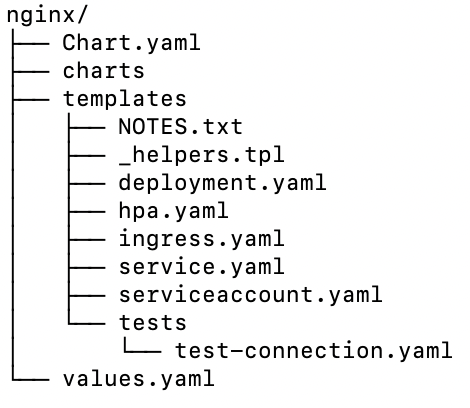
\includegraphics[width=0.5\columnwidth]{chart_struct.png}
    \caption{Helm Chart structure}
    \label{fig:chart_struct}
\end{figure}

Figure \ref{fig:chart_struct} presents an example of a Helm Chart directory. A Chart typically package these files:
\begin{itemize}
    \item \texttt{Chart.yaml}: a file that contains metadata about the chart.
    \item \texttt{values.yaml}: a file that contains the default values for a chart that will fill the templates.
    \item \texttt{templates/}: directory for template files. When Helm evaluates a chart, it will send all of the files in the \texttt{templates/} directory through the template rendering engine. It then collects the results of those templates and sends them on to Kubernetes.
    \item \texttt{templates/\_helpers.tpl}: a file that contains template helpers that can be re-used in other templates.
    \item \texttt{charts/}: a directory that contains the charts upon which the chart depends.
\end{itemize}

Users can customize the configuration of their application without needing to modify the chart by choosing to override the default values specified in the \texttt{values.yaml} file during chart installation. Charts are versioned, thus allowing easy upgrades, rollbacks and deletes with the \texttt{helm} CLI.

Helm Charts are often distributed on public Git repositories and/or Artifact Hub\footnote{\url{https://artifacthub.io}}. Coupled with Continuous Deployment tools such as Argo CD \cite{argocd} or Flux \cite{flux}, Helm is a powerful and one of the most used components in the DevOps toolchain.

\section{Methodology}

\subsection{Research Questions}

This study aims to improve our understanding of Helm Charts refactorings and the technical debts that occur in these projects. Accordingly, we answer the following research questions:
\begin{itemize}
    \item \textbf{RQ1:} What are the most common types of refactoring in Helm Charts?
    \item \textbf{RQ2:} What technical debts are they symptomatic of?
\end{itemize}

\subsection{Projects Selection}

We selected the Bitnami Helm Charts repository \cite{bitnami} as our subject of study. It is one of the most popular Helm Charts repository available on GitHub, providing charts for many popular applications.

They aim to offer a large choice of high quality updated production-ready Helm Charts and they have been around for more than 7 years, since the early days of Helm, making them a good candidate for our study.

\subsection{Refactoring Identification}

Using \textit{Pydriller} \cite{Spadini2018} we filtered all commits which message contains the substring \texttt{refactor} and with at least one template file or the \texttt{values.yaml} file modified.

With this method we managed to identify 35 commits across all Bitnami Helm Charts that are likely to be refactorings.

\subsection{Refactoring Classification}

With the help of the commit messages and changelogs, we manually analyzed each commit to list the major changes that were introduced. Once all changes were listed, we consolidated them into major refactoring types that must appear in at least two commits to be considered.

All commits have been checked by the sole author of this paper over the course of a week to ensure consistency while avoiding his weariness.

\section{Results}

Over the 35 identified commits, 9 of them were considered false positives (not enough changes, only documentation update, addition of new features, etc.).

With the remaining 26 commits, we identified 11 different types of major refactorings in Helm Charts. Each refactoring type has been classified into one technical debt that it is symptomatic of. Table \ref{tab:refactorings} provides a summary of our findings.

In the following subsections, we detail each of these refactorings with a focus on their impact on the quality of Helm Charts.

\begin{table*}
    \centering
    \caption{Helm Chart refactorings}
    \label{tab:refactorings}
    \begin{tabular}{cccc}
        \toprule
        \textbf{Refactoring Type}   & \textbf{Description}                                       & \textbf{Technical Debt} & \textbf{Commits Impacted} \\
        \midrule
        Named Template              & Update named template to reduce code duplication           & Maintainability         & 10                        \\
        Merge Resources             & Merge related resources to reduce the amount of manifests  & Maintainability         & 2                         \\
        Support Multiple Topologies & Support multiple deployment modes in the same chart        & Modularity              & 2                         \\
        Unhardcode Value            & Expose an existing hardcoded value in \texttt{values.yaml} & Modularity              & 7                         \\
        Expose Metrics              & Make the application easier to measure                     & Observability           & 2                         \\
        Update Labels/Annotations   & Update labels and annotations on the chart resources       & Observability           & 4                         \\
        Update Probes               & Update pod probes                                          & Observability           & 9                         \\
        Configure Security Context  & Setup Security Context for a Pod or a Container            & Security                & 3                         \\
        Rename Resource             & Rename a chart resource                                    & Understandability       & 5                         \\
        Reorder Spec                & Reorder the specification of a chart resource              & Understandability       & 2                         \\
        Reorganize Keys             & Reorganize the keys in \texttt{values.yaml}                & Understandability       & 13                        \\
        \bottomrule
    \end{tabular}
\end{table*}

\subsection{Maintainability-related Refactorings}

The three following refactorings are related to maintainability. As Kubernetes manifests can be quite verbose, Helm Charts tend to be large and complex. This can lead to code duplication and make the chart harder to maintain.

\subsubsection{Named Template}
Helm Charts are using Go templates \cite{gotpl} to generate Kubernetes manifests. Developers can define named templates that can be reused in other templates. This is very useful to avoid code duplication of common parts of the manifests such as labels, annotations, etc. (Figure \ref{fig:namedtpl})

\begin{figure}
    \begin{minted}[fontsize=\footnotesize,breaklines,linenos,numbersep=2pt,frame=single]{diff}
[templates/_helpers.tpl]
+{{/*
+Labels to use on daemonset.spec.selector.matchLabels, statefulset.spec.selector.matchLabels and svc.spec.selector
+*/}}
+{{- define "fluentd.matchLabels" -}}
+app.kubernetes.io/name: {{ include "fluentd.name" . }}
+app.kubernetes.io/instance: {{ .Release.Name }}
+{{- end -}}

[templates/forwarder-daemonset.yaml]
 spec:
   selector:
-    matchLabels:
-      app.kubernetes.io/name: {{ include "fluentd.name" . }}
-      app.kubernetes.io/instance: {{ .Release.Name }}
+    matchLabels: {{ include "fluentd.matchLabels" . | nindent 6 }}
    \end{minted}
    \caption{Named Template - Extract of commit \texttt{ddf4a5e}}
    \label{fig:namedtpl}
\end{figure}

\subsubsection{Merge Resources}
Helm Charts are often composed of multiple Kubernetes resources. In some cases, these resources are related to each other and can be merged into a single resource (e.g. multiple configmaps, secrets or even deployments and statefulsets). This can help reduce the amount of manifests and make the chart easier to maintain.

\subsection{Modularity-related Refactorings}

Modularity is an important aspect of Helm Charts. It allows users to easily customize the chart to their needs and reuse the chart across multiple projects. The following two refactorings are related to modularity.

\subsubsection{Support Multiple Topologies}
Some applications can be deployed in different topologies (e.g. standalone, distributed, etc.). In this case, it is useful to support multiple topologies in the same chart to avoid chart duplication and make the chart adaptable to different use cases.

\subsubsection{Unhardcode Value}
Helm Charts often contain hardcoded values that are not exposed in the \texttt{values.yaml} file. This makes it difficult for users to customize the chart to their needs. In this case, it is useful to expose the hardcoded value in the \texttt{values.yaml} file to make the chart more modular.

\subsection{Observability-related Refactorings}

In DevOps, observability of applications is critical to ensure the reliability of the infrastructure. The following three refactorings are related to this quality.

\subsubsection{Expose Metrics}
Charts author can add optional resources to expose metrics of the application to third party tools such as Prometheus \cite{prom}. This makes Helm Chart applications auto-discoverable by these tools and easier to monitor.

\subsubsection{Update Labels/Annotations}
Labels and annotations are used by Kubernetes to identify and group resources. Kubernetes recommends a set of labels and annotations to be used in the manifests \cite{reclabels}. They help developers to easily identify the resources and make the application easier to monitor and manage.

\subsubsection{Update Probes}
Liveness, Readiness and Startup Probes are used by Kubernetes to check the health of the application \cite{probes}. They are a powerful tool to make the application more resilient and self-healing. However, they must be configured properly to avoid excessive restarts and cascading failures. (Figure \ref{fig:probes})

\begin{figure}
    \begin{minted}[fontsize=\footnotesize,breaklines,linenos,numbersep=2pt,frame=single]{diff}
+ {{- if .Values.startupProbe.enabled }}
+ startupProbe:
+   httpGet:
+     path: {{ .Values.startupProbe.path }}
+     port: http
+   initialDelaySeconds: {{ .Values.startupProbe.initialDelaySeconds }}
+   periodSeconds: {{ .Values.startupProbe.periodSeconds }}
+   timeoutSeconds: {{ .Values.startupProbe.timeoutSeconds }}
+   successThreshold: {{ .Values.startupProbe.successThreshold }}
+   failureThreshold: {{ .Values.startupProbe.failureThreshold }}
+ {{- else if .Values.customStartupProbe }}
+ startupProbe: {{- include "common.tplvalues.render" (dict "value" .Values.customStartupProbe "context" $) | nindent 12 }}
+ {{- end }}
    \end{minted}
    \caption{Update Probes - Extract of commit \texttt{31bcd6}}
    \label{fig:probes}
\end{figure}

\subsection{Security-related Refactorings}

Today, security is a major concern for organizations and software deployments should be designed with security in mind. We observed one refactoring related to security in our study.

\subsubsection{Configure Security Context}
Security Context is a Kubernetes feature that allows users to define the security settings for a Pod or a Container \cite{secctx}. It includes settings such as the user ID, the group ID, the SELinux context, etc. Security Context can be used to make the application more secure and resilient by reducing the attack surface. (Figure \ref{fig:sc})

\begin{figure}
    \begin{minted}[fontsize=\footnotesize,breaklines,linenos,numbersep=2pt,frame=single]{diff}
[values.yaml]
+containerSecurityContext:
+  enabled: true
+  runAsUser: 1001
+  runAsNonRoot: true

[templates/cronjob.yaml]
 apiVersion: batch/v1beta1
 kind: CronJob
 spec:
   template:
     spec:
       template:
           containers:
             - name: etcd-snapshotter
               image: {{ include "etcd.image" . }}
               imagePullPolicy: {{ .Values.image.pullPolicy | quote }}
+              {{- if .Values.containerSecurityContext.enabled }}
+              securityContext: {{- omit .Values.containerSecurityContext "enabled" | toYaml | nindent 16 }}
+              {{- end }}
    \end{minted}
    \caption{Configure Security Context - Extract of commit \texttt{5741a6d}}
    \label{fig:sc}
\end{figure}

\subsection{Understandability-related Refactorings}

The following three refactorings are related to understandability. They help make the chart and underlying deployments easier to understand for users who want to deploy them.

\subsubsection{Rename Resource}
Like the name of a function in a program, the name of a Kubernetes resource should be meaningful and easy to understand. This makes it easier for users to identify the resources and understand their purpose.

\subsubsection{Reorder Spec}
Some Kubernetes resources such as \texttt{Deployment} and \texttt{StatefulSet} have a large number of fields in their specification \cite{apispec}. In this case, it is useful to reorder the fields in a logical order to make the manifest easier to understand.

\subsubsection{Reorganize Keys}
When the \texttt{values.yaml} file contains a large number of settable keys, it can be difficult for users to find the key they are looking for. In this case, it is useful to reorganize the keys in a logical order and group them by category to make the file easier to understand.

\vspace{1em}
\noindent
\fbox{\begin{minipage}{\columnwidth}
        \textbf{RQ1 Summary:} We observed 11 common types of refactorings in Helm Charts: Named Template, Merge Resources, Support Multiple Topologies, Unhardcode Value, Expose Metrics, Update Labels/Annotations, Update Probes, Configure Security Context, Rename Resource, Reorder Spec and Reorganize Keys.
    \end{minipage}}

\vspace{1em}
\noindent
\fbox{\begin{minipage}{\columnwidth}
        \textbf{RQ2 Summary:} Helm Charts refactorings are often associated with technical debt related to maintainability, modularity, observability, security or understandability.
    \end{minipage}}

\section{Threats to Validity}

Due to its empirical nature, our study findings are exposed to some potential threats to validity.

\subsection{Construct Validity}

Construct validity refers to the degree to which the operational definitions of the study variables are accurate representations of the theoretical constructs.

In our study, we used the commit messages and changelogs to identify the refactorings. However, these messages are not always accurate and may not reflect the actual changes made in the commit. To mitigate this threat, we manually analyzed each commit to ensure the accuracy of our findings. However, 1) manual analysis is time-consuming and quite subjective (even more when done by a single person) and 2) we still may have missed some refactorings that were not referenced in the commit messages.

\subsection{Internal Validity}

Internal validity refers to the degree to which the observed effects are caused by the treatment in the study.

Due to time constraints we only analyzed a single chart repository. This may limit the generalizability of our findings. However, we believe that our findings are still relevant as the Bitnami repository is one of the most popular and largest Helm Charts repository available on GitHub and is still actively maintained as of today.

\subsection{External Validity}

External validity refers to the degree to which the results of the study can be generalized to other contexts.

This study focuses on Helm Charts and may not be applicable to other types of Kubernetes deployments.

\section{Related Works}

A study conducted by Rahman and al. \cite{rahman2023security} identified security misconfigurations in Kubernetes manifests. Our research did found \textit{Configure Security Context} refactorings which are a response to one of their misconfiguration categories.

Another work of Zerouali and al. \cite{zerouali2022helm} points out the outdateness and security risks that can appear in Helm Charts, with an emphasis on used container images and chart dependencies. While our results are out of scope with this study, we recommend practitioners a look at their findings to improve chart security.

As Kubernetes use Docker container images for deployments, Ksontini and al. \cite{kessentini2021refactorings} findings on refactoring and technical debt for Docker projects provide further insights on this underlying layer of Helm Chart deployments.

\section{Conclusion}

In this paper, we presented a study of the technical debt and refactorings incurred in the development and maintenance of reusable Helm Charts. We analyzed the evolution of Helm Charts in the Bitnami repository and manually identified 11 common patterns of refactorings. These refactorings are often associated with technical debt related to maintainability, modularity, observability, security or understandability.

Our findings can help developers and organizations improve the quality of their Helm Charts by adopting best practices that would avoid the need for refactorings and breaking changes in the first place.

\bibliographystyle{IEEEtran}
\bibliography{IEEEabrv,references.bib}

\end{document}
